%%%%%%%%%%%%%%%%%%%%%%%%%%%%%%%%%%%%

\section{数値データの分析}

%%%%%%%%%%%%%%%%%%%%%%%%%%%%%%%%%%%%

\subsection{対データの散布図}

%%%%%%%%%%%%%%%%%%%%%%%%%%%%%%%%%%%%

\begin{frame}
\frametitle{散布図}

\hl{散布図}は2つの数値変数間の関係を可視化するのに有用である。

\begin{columns}[c]

\column{0.6 \textwidth}

\dq{平均寿命と合計特殊出生率は\hl{関連がある}か、それとも\hl{独立}か？}

\soln{線形かつ負の関連があるように見える：出生率が上がるにつれ、平均寿命が下がる。}

\dq{この関係は年代を通じて変わらなかったか、それとも変化したか？}

\soln{関係は年代とともに変化した。}

\column{0.4 \textwidth}

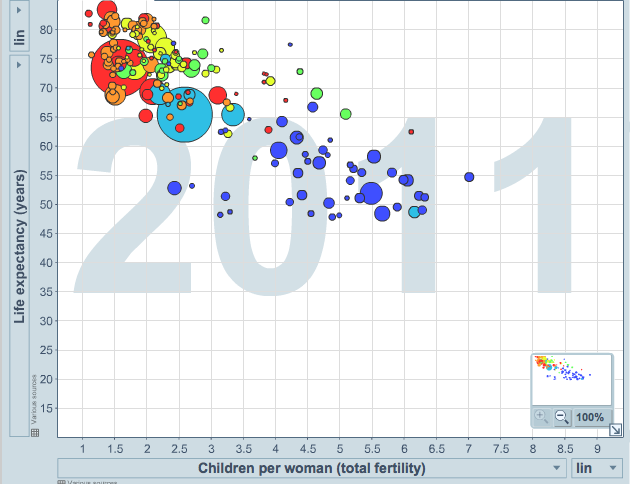
\includegraphics[width=\textwidth]{2-1_numerical_data/figures/life_exp_child}

\end{columns}

\ct{\webURL{http://www.gapminder.org/world}}

\end{frame}

%%%%%%%%%%%%%%%%%%%%%%%%%%%%%%%%%%%%

\subsection{ドットプロットと平均}

%%%%%%%%%%%%%%%%%%%%%%%%%%%%%%%%%%%%

\begin{frame}
\frametitle{ドットプロット}

1つの数値変数を可視化するのに有用。色が濃い部分はより多くの観測値が集中している。

\begin{center}
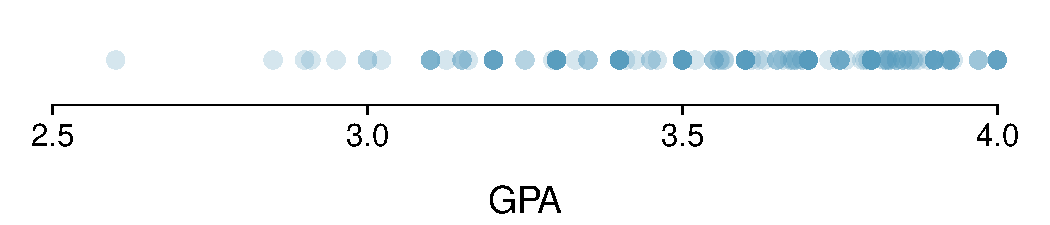
\includegraphics[width=\textwidth]{2-1_numerical_data/figures/gpa_dot_plot/gpa_dot_plot}
\end{center}

\dq{このデータセットのGPAの分布をどのように説明するか？分布の中心・形状・散らばりについて述べること。}

\end{frame}

%%%%%%%%%%%%%%%%%%%%%%%%%%%%%%%%%%%%

\begin{frame}
\frametitle{ドットプロットと平均}

\begin{center}
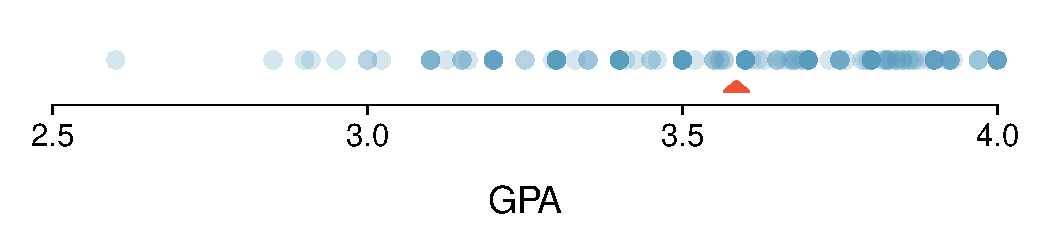
\includegraphics[width=\textwidth]{2-1_numerical_data/figures/gpa_dot_plot/gpa_dot_plot_mean}
\end{center}

\begin{itemize}

\item \hl{平均}（上のプロットで三角形で示されている）は、データの\hl{分布}の中心を測る方法の1つである。

\item GPAの平均は3.59である。

\end{itemize}

\end{frame}

%%%%%%%%%%%%%%%%%%%%%%%%%%%%%%%%%%%%

\begin{frame}
\frametitle{平均}

\begin{itemize}

\item \hl{標本平均}（\mathhl{\bar{x}} で表す）は次のように計算できる：

\[ \bar{x} = \frac{x_1 + x_2 + \cdots + x_n}{n}, \]

ここで $x_1, x_2, \cdots, x_n$ は \hl{n} 個の観測値を表す。

\item \hl{母平均}も同様に計算されるが \mathhl{\mu} で表される。母集団データが得られることはまれなため、$\mu$ を計算することはしばしば不可能である。

\item 標本平均は\hl{標本統計量}であり、母平均の\hl{点推定値}として機能する。この推定は完璧ではないかもしれないが、標本が良好（母集団を代表している）であれば、通常は十分な推定値となる。

\end{itemize}

\end{frame}

%%%%%%%%%%%%%%%%%%%%%%%%%%%%%%%%%%%%

\begin{frame}
\frametitle{積み上げドットプロット}

棒が高い部分はより多くの観測値が集中しており、分布の中心と形状をやや判断しやすくなる。

\begin{center}

\includegraphics[width=\textwidth]{2-1_numerical_data/figures/gpa_dot_plot/gpa_dot_plot_stacked}
\end{center}

\end{frame}

%%%%%%%%%%%%%%%%%%%%%%%%%%%%%%%%%%%%

\subsection{ヒストグラムと分布の形状}

%%%%%%%%%%%%%%%%%%%%%%%%%%%%%%%%%%%%

\begin{frame}[fragile]
\frametitle{ヒストグラム―課外活動時間}

\begin{itemize}

\item ヒストグラムは\hl{データの密度}を表す。棒が高い部分はデータが相対的に多い。

\item ヒストグラムはデータ分布の\hl{形状}を説明するのに特に便利である。

\item 選択する\hl{階級幅}によってヒストグラムが示す内容が変わる。

\end{itemize}

\begin{center}
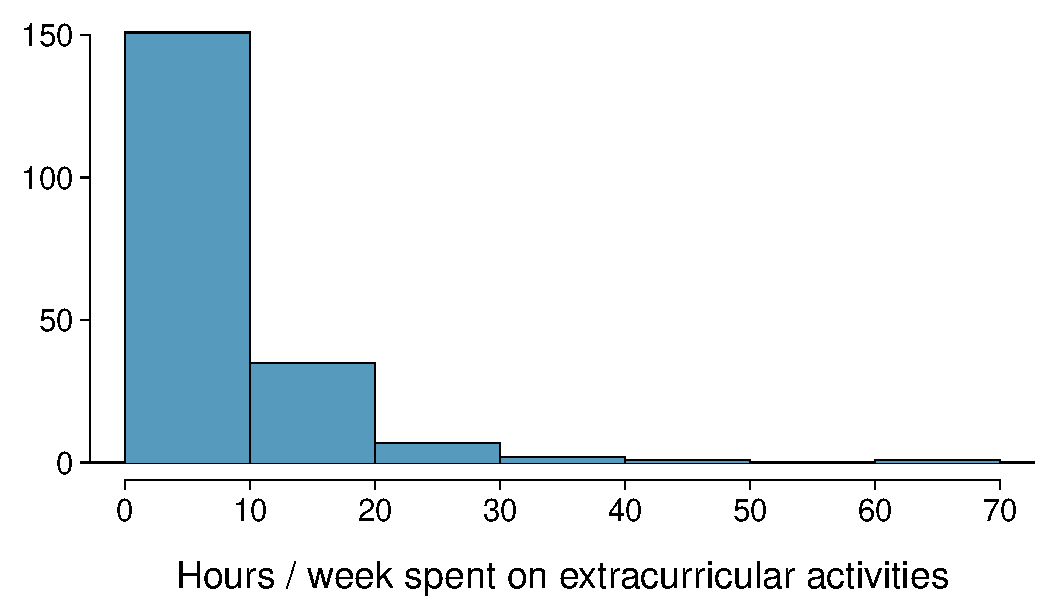
\includegraphics[width=0.65\textwidth]{2-1_numerical_data/figures/extracurr_hrs_hist/extracurr_hrs_hist}
\end{center}

\end{frame}

%%%%%%%%%%%%%%%%%%%%%%%%%%%%%%%%%%%%

\begin{frame}
\frametitle{階級幅}

\dq{これらのヒストグラムのうち有用なものはどれか？データを明かしすぎているのはどれか？隠しすぎているのはどれか？}

\begin{center}
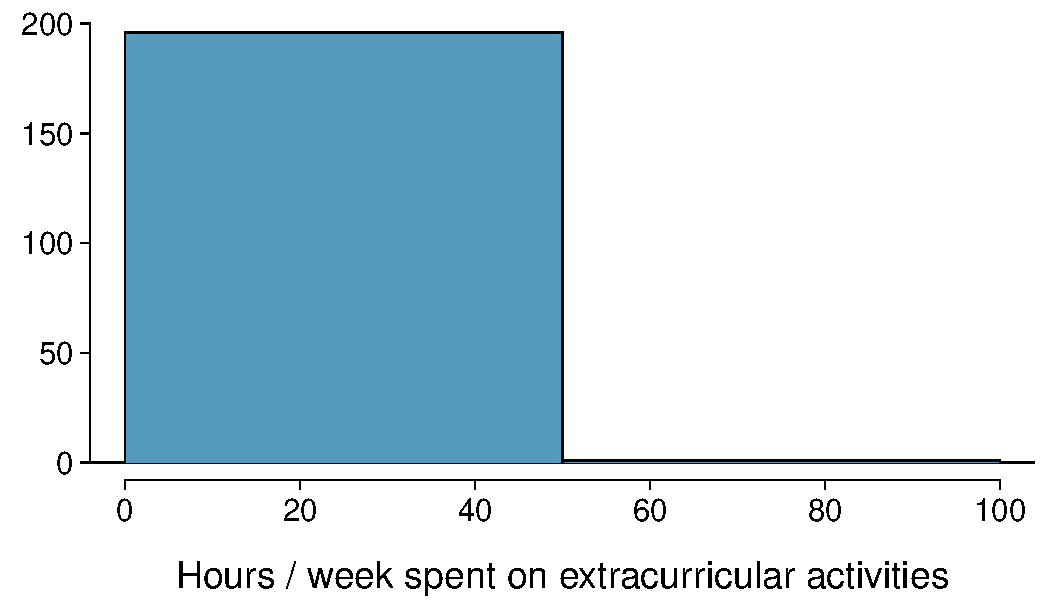
\includegraphics[width=0.45\textwidth]{2-1_numerical_data/figures/extracurr_hrs_hist/extracurr_hrs_hist2}
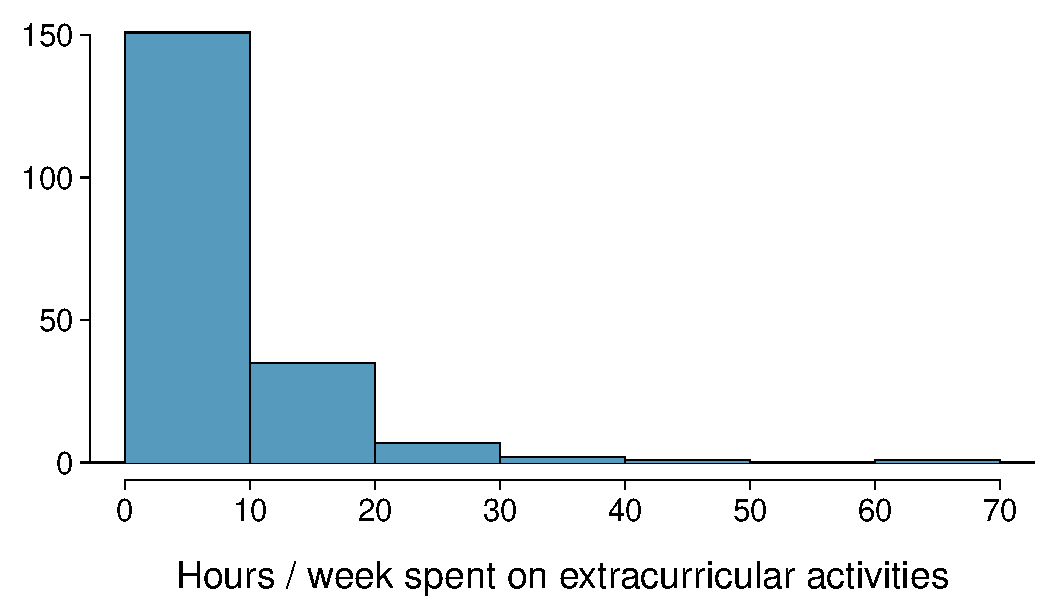
\includegraphics[width=0.45\textwidth]{2-1_numerical_data/figures/extracurr_hrs_hist/extracurr_hrs_hist} \\
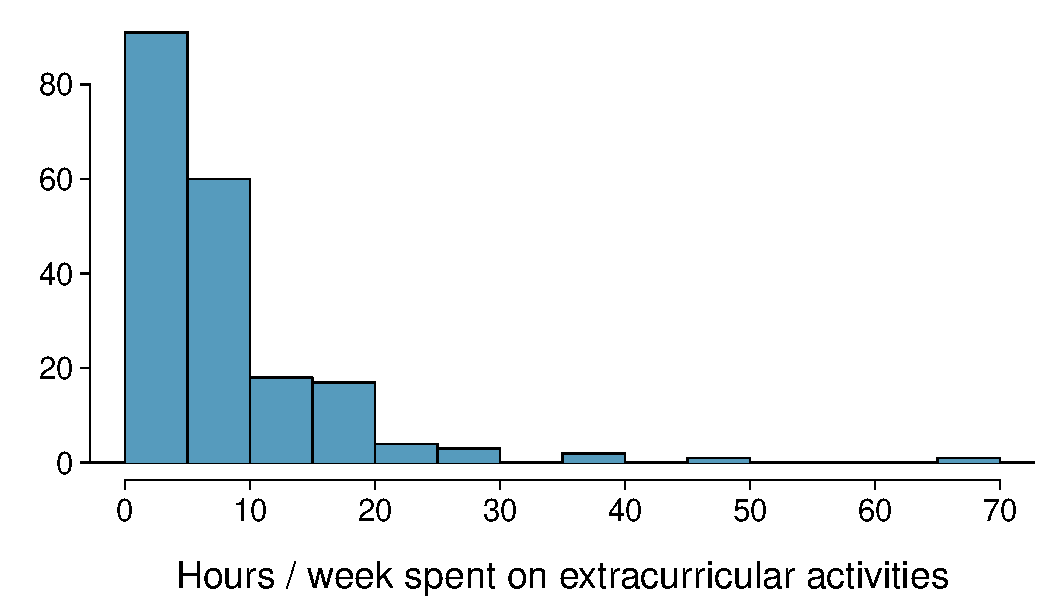
\includegraphics[width=0.45\textwidth]{2-1_numerical_data/figures/extracurr_hrs_hist/extracurr_hrs_hist20}
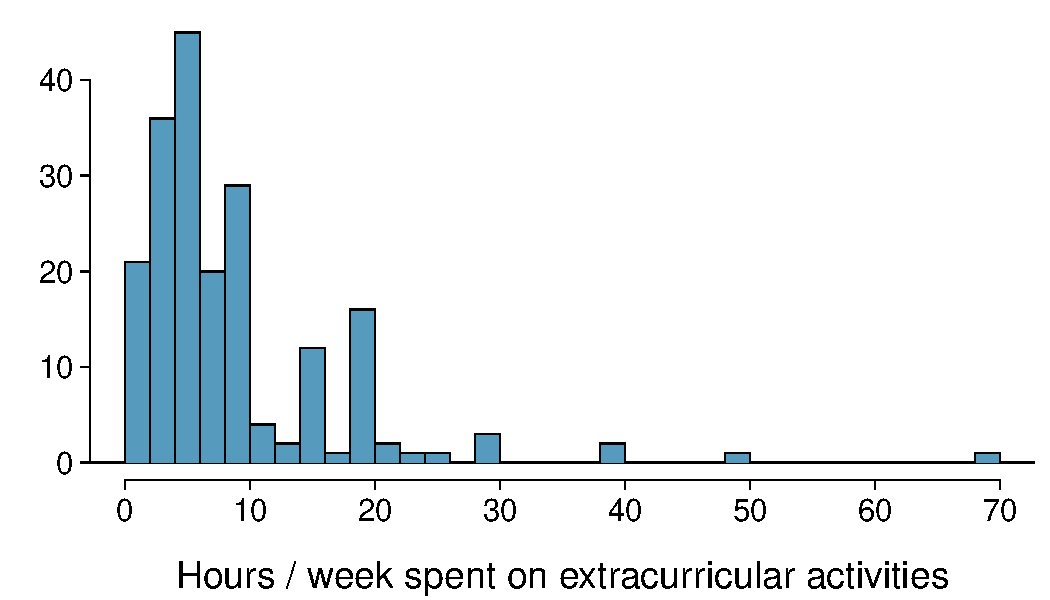
\includegraphics[width=0.45\textwidth]{2-1_numerical_data/figures/extracurr_hrs_hist/extracurr_hrs_hist30}
\end{center}

\end{frame}

%%%%%%%%%%%%%%%%%%%%%%%%%%%%%%%%%%%%

\begin{frame}
\frametitle{分布の形状：最頻値の個数}

ヒストグラムに1つの顕著な山（\hl{単峰型}）、複数の顕著な山（\hl{二峰型・多峰型}）、または顕著な山がない（\hl{一様型}）か？

\begin{center}
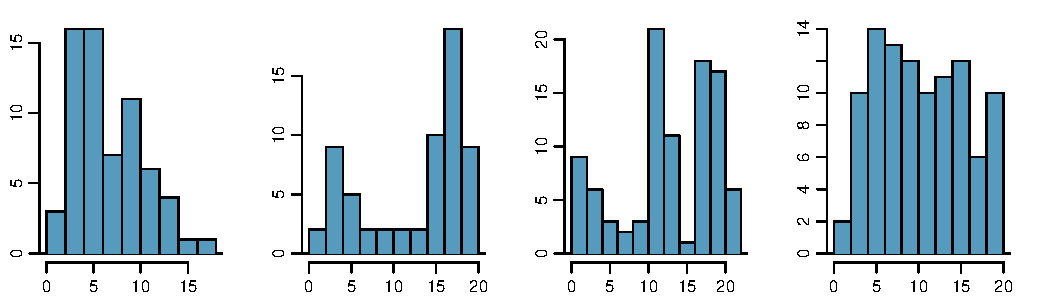
\includegraphics[width=0.75\textwidth]{2-1_numerical_data/figures/singleBiMultiModalUnifPlots/singleBiMultiModalUnifPlots}
\end{center}

\Note{最頻値の個数を判断するには、ヒストグラムの上に滑らかな曲線を描くことを想像しよう――棒を木のブロックと見立て、そこにスパゲッティを垂らしたときの形が滑らかな曲線になる。}

\end{frame}

%%%%%%%%%%%%%%%%%%%%%%%%%%%%%%%%%%%%

\begin{frame}
\frametitle{分布の形状：歪み}

ヒストグラムは\hl{右歪み}か、\hl{左歪み}か、それとも\hl{対称}か？

\begin{center}
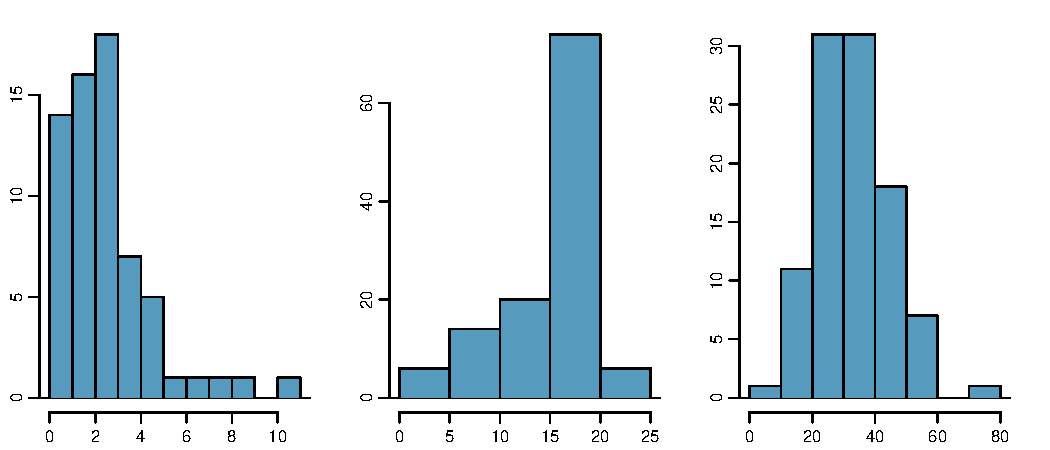
\includegraphics[width=0.8\textwidth]{2-1_numerical_data/figures/skewedSymPlots/skewedSymPlots}
\end{center}

\Note{ヒストグラムは長い裾の側に歪んでいると言う。}

\end{frame}

%%%%%%%%%%%%%%%%%%%%%%%%%%%%%%%%%%%%

\begin{frame}
\frametitle{分布の形状：異常値}

異常な観測値や潜在的な\hl{外れ値}はあるか？

\begin{center}
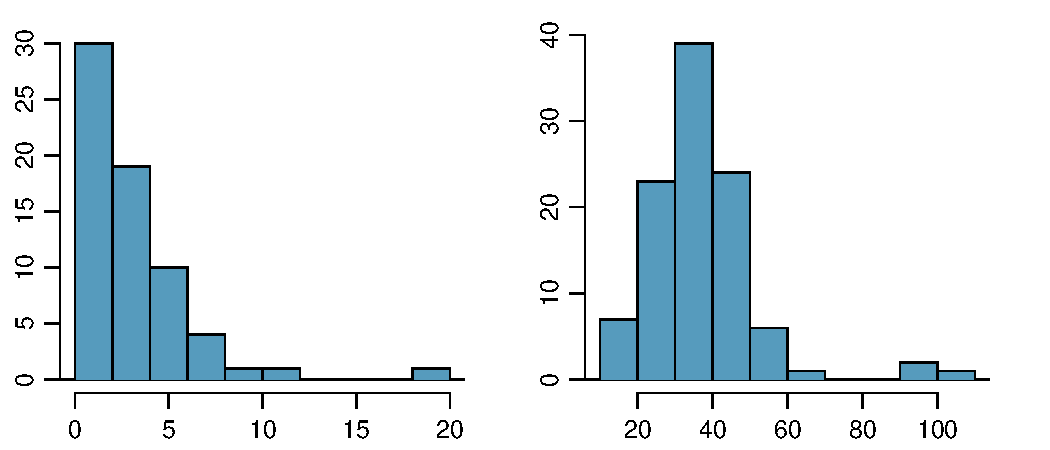
\includegraphics[width=0.8\textwidth]{2-1_numerical_data/figures/outlierPlots/outlierPlots}
\end{center}

\end{frame}

%%%%%%%%%%%%%%%%%%%%%%%%%%%%%%%%%%%%

\begin{frame}
\frametitle{課外活動}

\dq{学生が課外活動に費やす週当たりの時間の分布の形状をどのように説明するか？}

\begin{center}
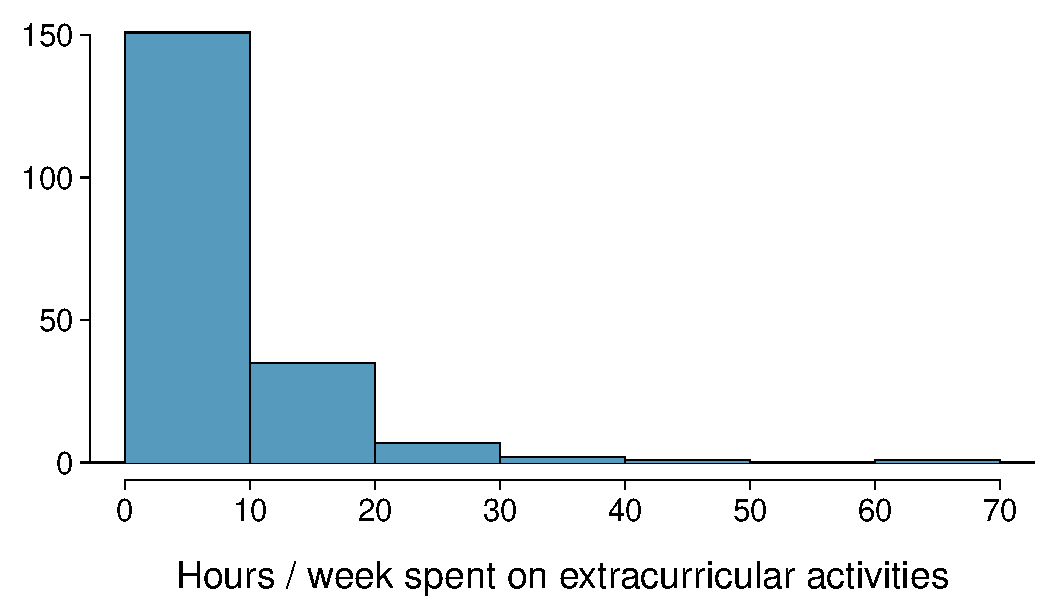
\includegraphics[width=0.75\textwidth]{2-1_numerical_data/figures/extracurr_hrs_hist/extracurr_hrs_hist}
\end{center}

\soln{単峰型・右歪みで、週60時間に潜在的な異常値がある。}

\end{frame}

%%%%%%%%%%%%%%%%%%%%%%%%%%%%%%%%%%%%

\begin{frame}
\frametitle{よく見られる分布の形状}

\begin{itemize}

\item 最頻値の個数 \\
$\:$ \\

\begin{columns}[c]
\column{0.25\textwidth}
単峰型 \\
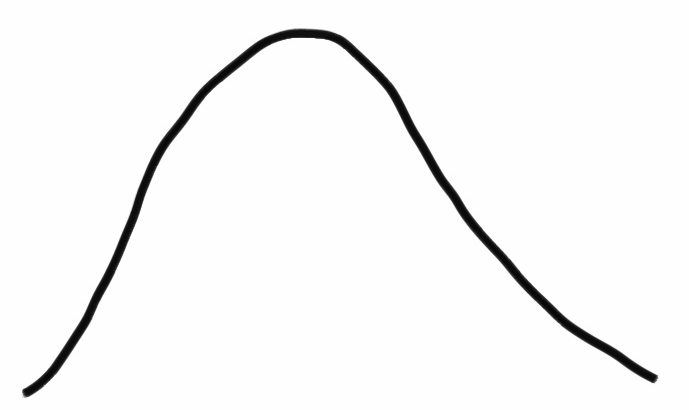
\includegraphics[width=\textwidth]{2-1_numerical_data/figures/shape_sketches/unimodal}
\column{0.25\textwidth}
二峰型 \\
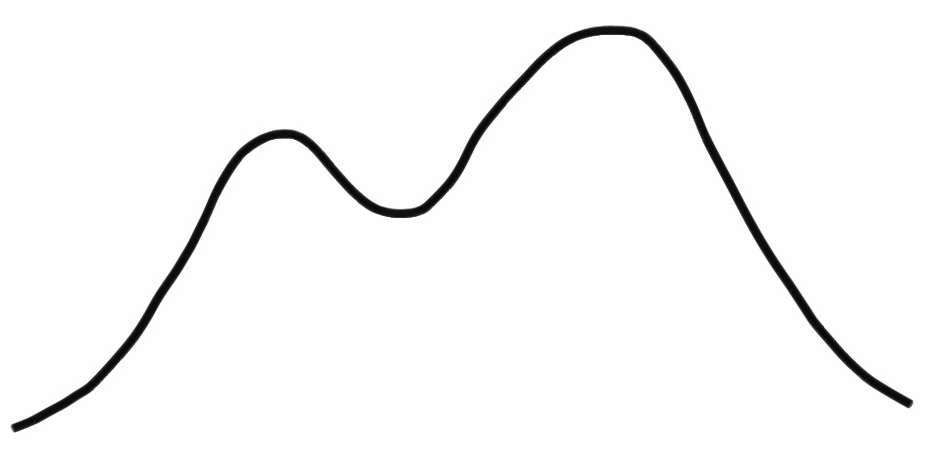
\includegraphics[width=\textwidth]{2-1_numerical_data/figures/shape_sketches/bimodal}
\column{0.25\textwidth}
多峰型 \\
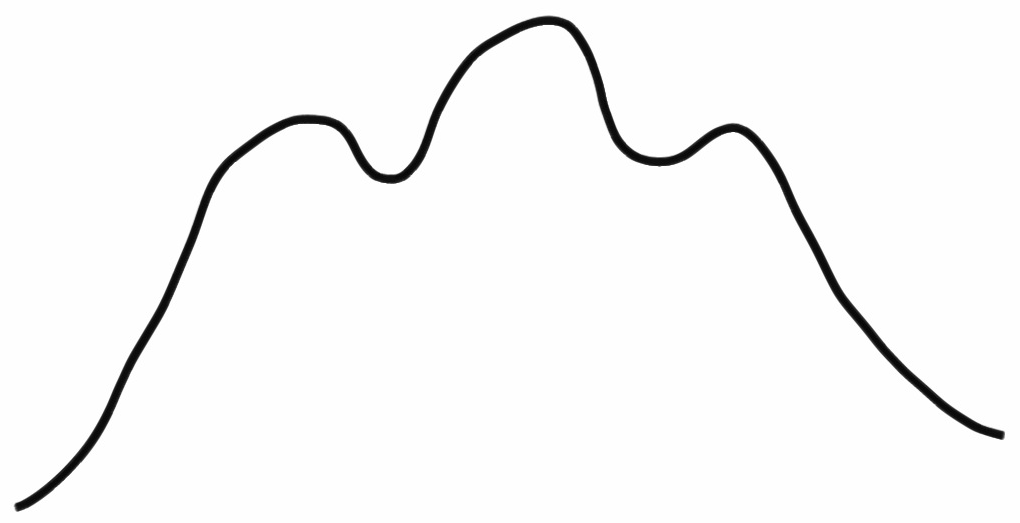
\includegraphics[width=\textwidth]{2-1_numerical_data/figures/shape_sketches/multimodal}
\column{0.25\textwidth}
一様型
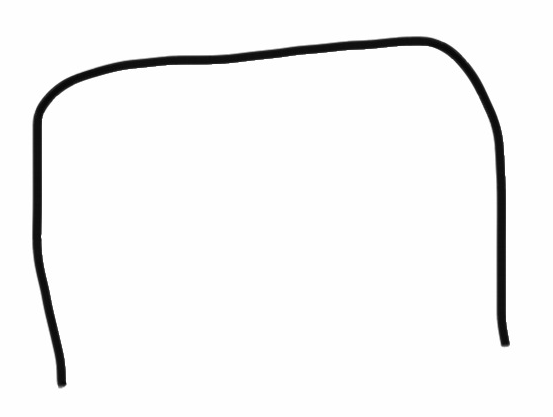
\includegraphics[width=\textwidth]{2-1_numerical_data/figures/shape_sketches/uniform}
\end{columns}

$\:$ \\

\item 歪み \\
$\:$ \\

\begin{columns}[c]
\column{0.25\textwidth}
右歪み \\
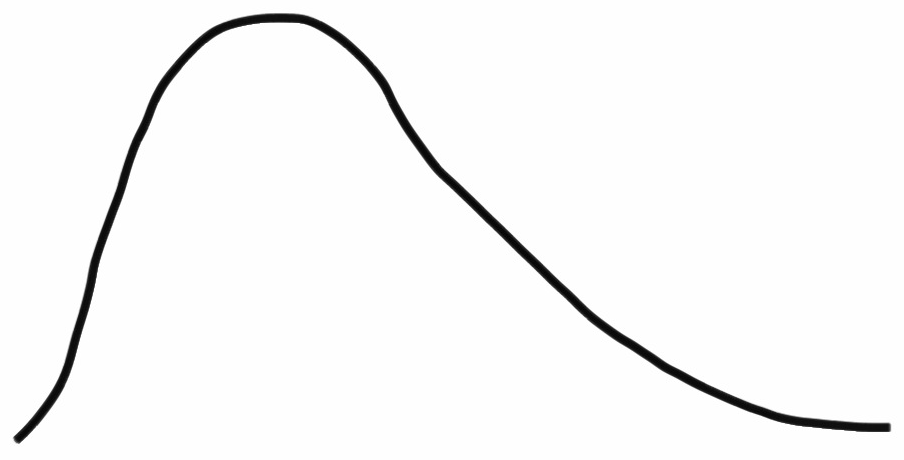
\includegraphics[width=\textwidth]{2-1_numerical_data/figures/shape_sketches/right_skew}
\column{0.25\textwidth}
左歪み \\
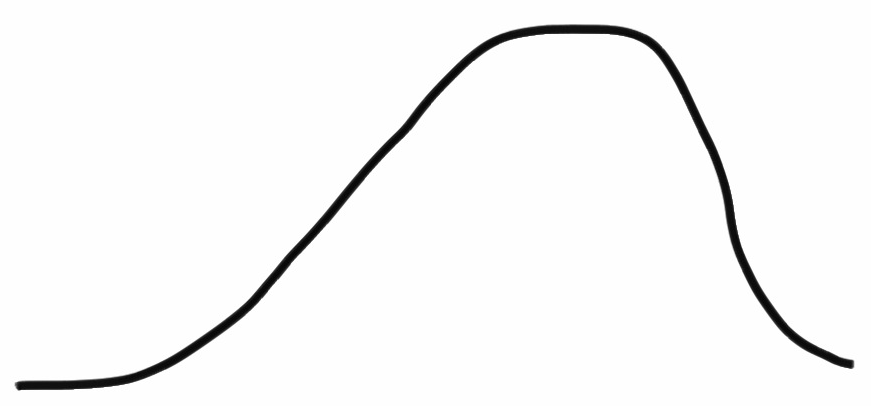
\includegraphics[width=\textwidth]{2-1_numerical_data/figures/shape_sketches/left_skew}
\column{0.25\textwidth}
対称 \\
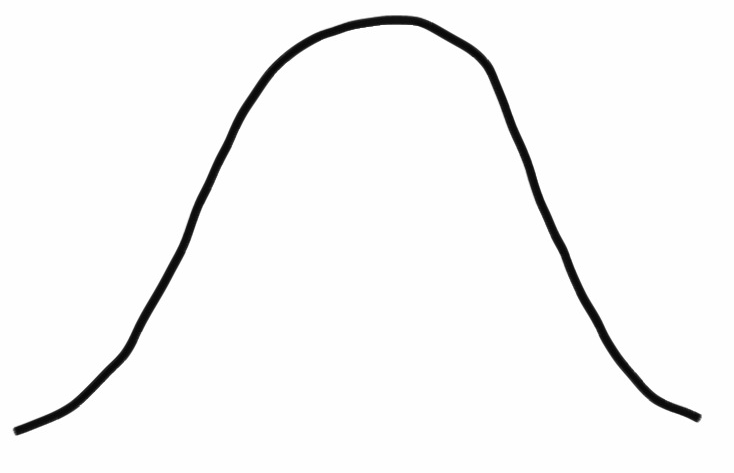
\includegraphics[width=\textwidth]{2-1_numerical_data/figures/shape_sketches/symmetric}
\end{columns}

\end{itemize}

\end{frame}

%%%%%%%%%%%%%%%%%%%%%%%%%%%%%%%%%%%

\begin{frame}
\frametitle{練習問題}

\pq{次の変数のうち一様分布すると予想されるものはどれか？}

\begin{enumerate}[(a)]
\item 成人女性の体重
\item ノースカロライナ州の無作為標本の給与
\item 住宅価格
\solnMult{クラスメートの誕生日（日付）}
\end{enumerate}

\end{frame}

%%%%%%%%%%%%%%%%%%%%%%%%%%%%%%%%%%%

\begin{frame}
\frametitle{応用活動：分布の形状}

\app{次の変数の予想される分布をスケッチせよ：
\begin{itemize}
\item ピアスの数
\item 試験の得点
\item IQスコア
\end{itemize}
任意の変数の予想分布を判断する方法を簡潔に（1〜2文で）説明せよ。
}

\end{frame}

%%%%%%%%%%%%%%%%%%%%%%%%%%%%%%%%%%%

\begin{frame}
\frametitle{あなたは「典型的な」人か？}

\begin{center}
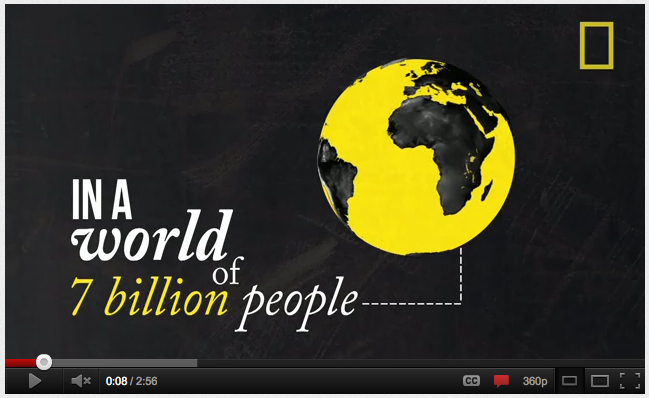
\includegraphics[width=0.75\textwidth]{2-1_numerical_data/figures/typical}
\end{center}

\begin{center}
\footnotesize{\webURL{http://www.youtube.com/watch?v=4B2xOvKFFz4}}
\end{center}

\dq{分布の真の特徴を伝えるうえで、中心だけがどれほど有用か？}

\end{frame}

%%%%%%%%%%%%%%%%%%%%%%%%%%%%%%%%%%%%

\subsection{分散と標準偏差}

%%%%%%%%%%%%%%%%%%%%%%%%%%%%%%%%%%%

\begin{frame}
\frametitle{分散}

\hl{分散}は平均からの偏差の2乗のおおよその平均である。

\formula{
\[ s^2 = \frac{\sum_{i = 1}^n (x_i - \bar{x})^2}{n - 1} \]
}

\twocol{0.5}{0.5}
{
\begin{itemize}

\item 標本平均は $\bar{x} = 6.71$、標本サイズは $n = 217$ である。

\item 学生が1晩に睡眠をとる時間の分散は次のように計算できる：

\end{itemize}
}
{
\begin{center}
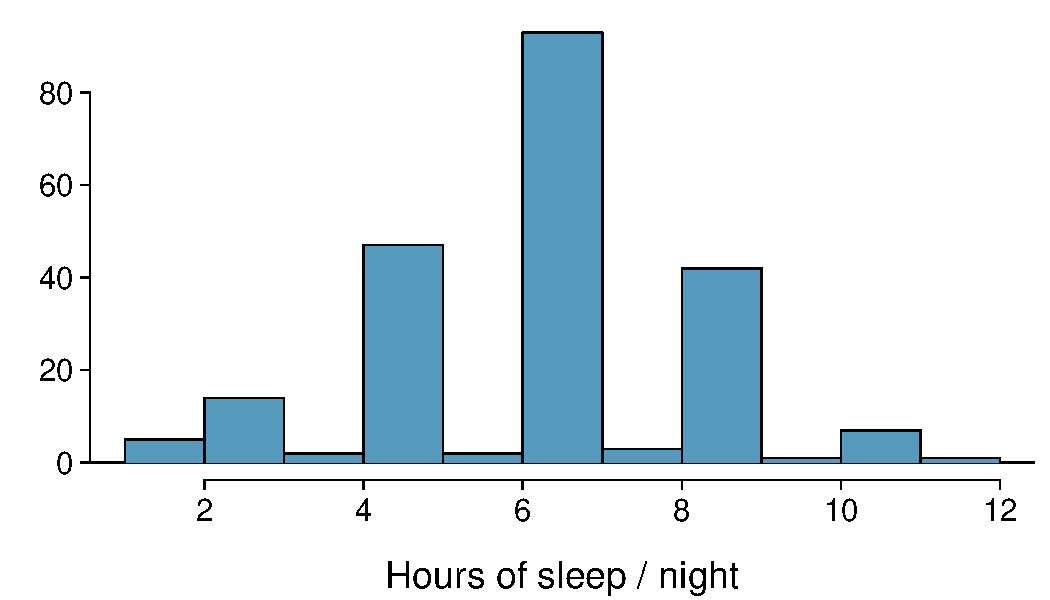
\includegraphics[width=\textwidth]{2-1_numerical_data/figures/sleep_hist/sleep_hist}
\end{center}
}
$\:$
\[ s^2 = \frac{(5 - 6.71)^2 + (9 - 6.71)^2 + \cdots + (7 - 6.71)^2}{217 - 1} = 4.11~\text{時間}^2 \]

\end{frame}

%%%%%%%%%%%%%%%%%%%%%%%%%%%%%%%%%%%

\begin{frame}
\frametitle{分散（続き）}

\dq{なぜ分散の計算に偏差の2乗を使うのか？}

\soln{
\begin{itemize}
\item 負の値をなくし、平均から等距離の観測値が等しく重み付けされるようにするため。
\item より大きな偏差を重く扱うため。
\end{itemize}
}

\end{frame}

%%%%%%%%%%%%%%%%%%%%%%%%%%%%%%%%%%

\begin{frame}
\frametitle{標準偏差}

\hl{標準偏差}は分散の平方根であり、データと同じ単位を持つ。

\formula{
\[ s = \sqrt{s^2} \]
}

\twocol{0.5}{0.5}
{
\begin{itemize}

\item 学生が1晩に睡眠をとる時間の標準偏差は次のように計算できる：
\[ s = \sqrt{4.11} = 2.03~\text{時間}\]

\item すべてのデータが平均の3標準偏差以内にあることが分かる。

\end{itemize}
}
{
\begin{center}
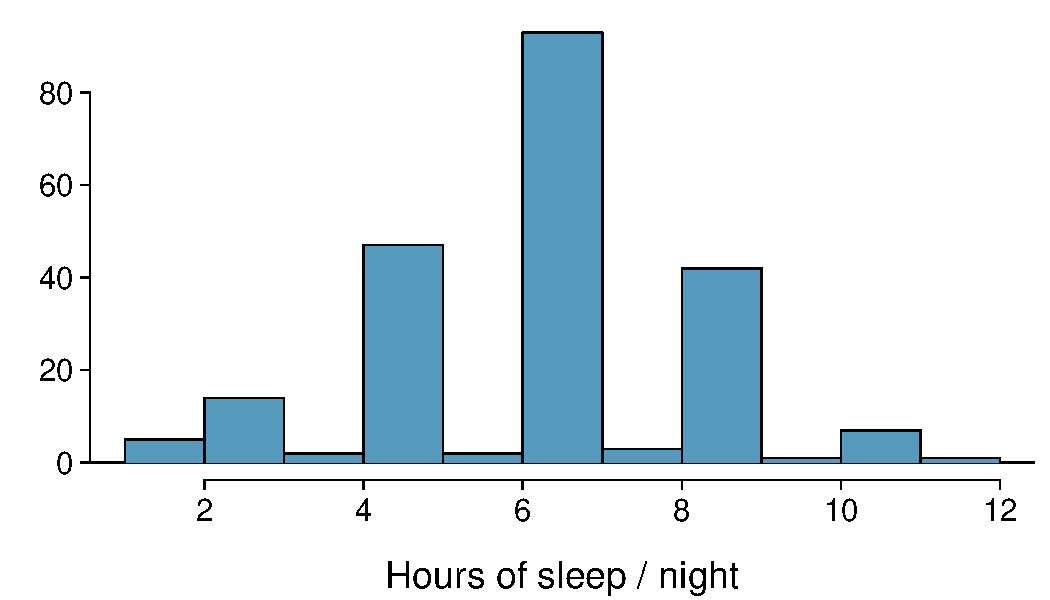
\includegraphics[width=\textwidth]{2-1_numerical_data/figures/sleep_hist/sleep_hist}
\end{center}
}

\end{frame}

%%%%%%%%%%%%%%%%%%%%%%%%%%%%%%%%%%%%

\subsection{箱ひげ図・四分位数・中央値}

%%%%%%%%%%%%%%%%%%%%%%%%%%%%%%%%%%%%

\begin{frame}
\frametitle{中央値}

\begin{itemize}

\item \hl{中央値}は、データを昇順に並べたときに真ん中を2分割する値である。

\[ 0,1,\orange{2},3,4 \]

\item 観測値の数が偶数の場合、中央値は真ん中2つの値の平均である。

\[ 0,1,\underline{2,3},4,5 \rightarrow \frac{2 + 3}{2} = \orange{2.5} \]

\item 中央値はデータの中間点であるため、値の50\%がその下にある。したがって、\hl{第50パーセンタイル}とも呼ばれる。

\end{itemize}

\end{frame}

%%%%%%%%%%%%%%%%%%%%%%%%%%%%%%%%%%%%

\begin{frame}[fragile]
\frametitle{Q1、Q3、IQR}

\begin{itemize}

\item 第25パーセンタイルは\hl{第1四分位数（Q1）}とも呼ばれる。

\item 第50パーセンタイルは中央値とも呼ばれる。

\item 第75パーセンタイルは\hl{第3四分位数（Q3）}とも呼ばれる。

\item Q1とQ3の間にはデータの中央50\%がある。このデータが示す範囲を\hl{四分位範囲（IQR）}と呼ぶ。
\formula{\[ IQR = Q3 - Q1 \]}
\end{itemize}

\end{frame}

%%%%%%%%%%%%%%%%%%%%%%%%%%%%%%%%%%%%

\begin{frame}
\frametitle{箱ひげ図}

\hl{箱ひげ図}の箱はデータの中央50\%を表し、箱内の太線は中央値である。

\begin{center}
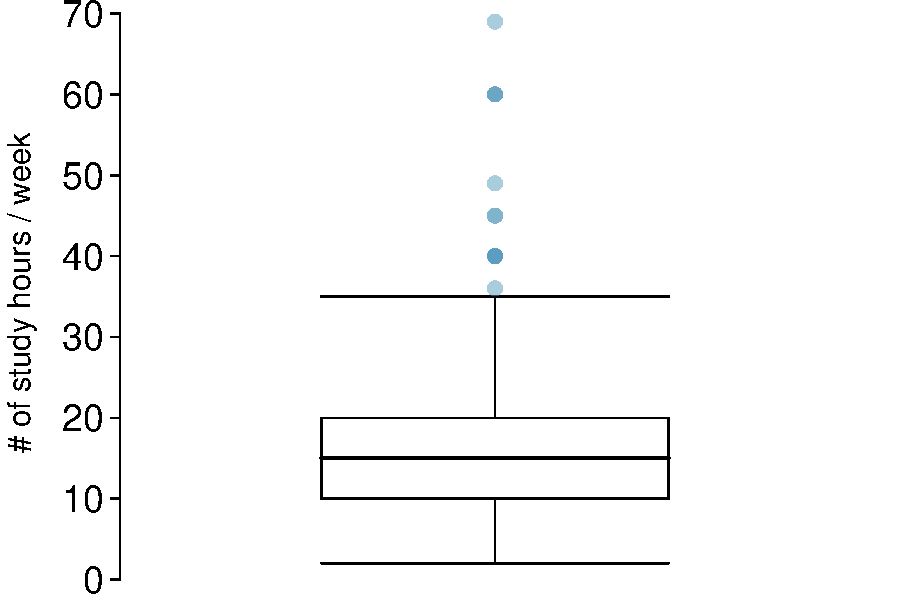
\includegraphics[width=0.7\textwidth]{2-1_numerical_data/figures/study_hours/study_hours_box}
\end{center}

\end{frame}

%%%%%%%%%%%%%%%%%%%%%%%%%%%%%%%%%%%%

\begin{frame}
\frametitle{箱ひげ図の構造}

\begin{center}
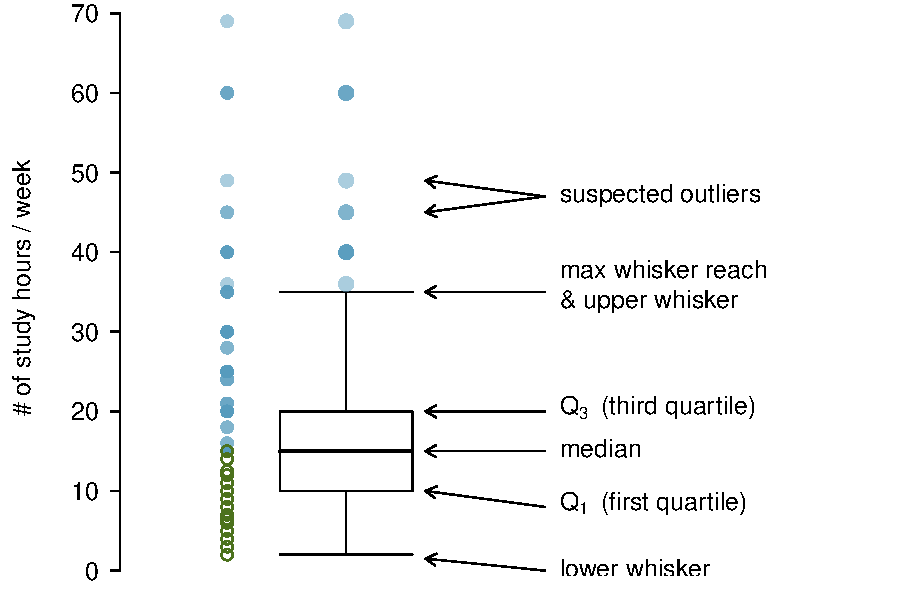
\includegraphics[width=0.95\textwidth]{2-1_numerical_data/figures/study_hours/study_hours_box_layout}
\end{center}

\end{frame}

%%%%%%%%%%%%%%%%%%%%%%%%%%%%%%%%%%%%

\begin{frame}[fragile]
\frametitle{ひげと外れ値}

\begin{itemize}

\item 箱ひげ図の\hl{ひげ}は四分位数から最大 $1.5 \times IQR$ まで伸びる。
\formula{
\vspace{-0.5cm}
\begin{align*}
\text{上ひげの最大リーチ} &= Q3 + 1.5 \times IQR \\
\text{下ひげの最大リーチ} &= Q1 - 1.5 \times IQR
\end{align*}
}
\vspace{-0.5cm}
{\small
\begin{align*}
IQR&: 20 - 10 = 10 \\
\text{上ひげの最大リーチ}&= 20 + 1.5 \times 10 = 35 \\
\text{下ひげの最大リーチ}&= 10 - 1.5 \times 10 = -5
\end{align*}
}

\vspace{-0.25cm}
\item 潜在的な\hl{外れ値}とは、ひげの最大リーチを超えた観測値である。残りのデータに対して極端に見える観測値である。

\end{itemize}

\end{frame}

%%%%%%%%%%%%%%%%%%%%%%%%%%%%%%%%%%%%

\begin{frame}
\frametitle{外れ値（続き）}

\dq{外れ値を探すことがなぜ重要か？}

\soln{
\begin{itemize}
\item 分布の極端な歪みを特定する。
\item データ収集・入力エラーを特定する。
\item データの興味深い特徴への洞察を得る。
\end{itemize}
}

\end{frame}

%%%%%%%%%%%%%%%%%%%%%%%%%%%%%%%%%%%%

\subsection{頑健な統計量}

%%%%%%%%%%%%%%%%%%%%%%%%%%%%%%%%%%%%

\begin{frame}
\frametitle{極端な観測値}

\dq{世帯収入の平均・中央値・標準偏差・IQRは、最大値を1,000万ドルに置き換えた場合どのように変化するか？最小値を1,000万ドルに置き換えた場合はどうか？}

\begin{center}

\includegraphics[width=\textwidth]{2-1_numerical_data/figures/house_income/house_income_dot_stacked}
\end{center}

\end{frame}

%%%%%%%%%%%%%%%%%%%%%%%%%%%%%%%%%%%%

\begin{frame}[shrink=10]
\frametitle{頑健な統計量}

\begin{center}

\includegraphics[width=0.9\textwidth]{2-1_numerical_data/figures/house_income/house_income_dot_stacked}
\end{center}

{\small
\begin{center}
\begin{tabular}{l c cc c cc}
  \hline
& \hspace{0mm} & \multicolumn{2}{c}{\bf 頑健} & \hspace{2mm} & \multicolumn{2}{c}{\bf 非頑健} \\
シナリオ && 中央値 & IQR && $\bar{x}$ & $s$ \\
  \hline
元のデータ && 19万 & 20万 && 24.5万 & 22.6万 \\
最大値を1,000万ドルに変更 && 19万 & 20万 && 30.9万 & 85.3万 \\
最小値を1,000万ドルに変更 && 20万 & 20万 && 31.6万 & 85.4万 \\
   \hline
\end{tabular}
\end{center}
}

\end{frame}

%%%%%%%%%%%%%%%%%%%%%%%%%%%%%%%%%%%%

\begin{frame}
\frametitle{頑健な統計量}

中央値とIQRは、平均と標準偏差よりも歪みや外れ値に対して頑健である。したがって、

\begin{itemize}
\item 歪んだ分布では、中心と散らばりを説明するために中央値とIQRを使う方が有用なことが多い
\item 対称な分布では、中心と散らばりを説明するために平均と標準偏差を使う方が有用なことが多い
\end{itemize}

$\:$ \\

\dq{学生の典型的な世帯収入を推定したい場合、平均と中央値のどちらに注目するか？}

\soln{中央値}

\end{frame}

%%%%%%%%%%%%%%%%%%%%%%%%%%%%%%%%%%%%

\begin{frame}[shrink=10]
\frametitle{平均と中央値}

\begin{itemize}

\item 分布が対称な場合、中心はしばしば平均として定義される：平均 $\approx$ 中央値

\begin{center}
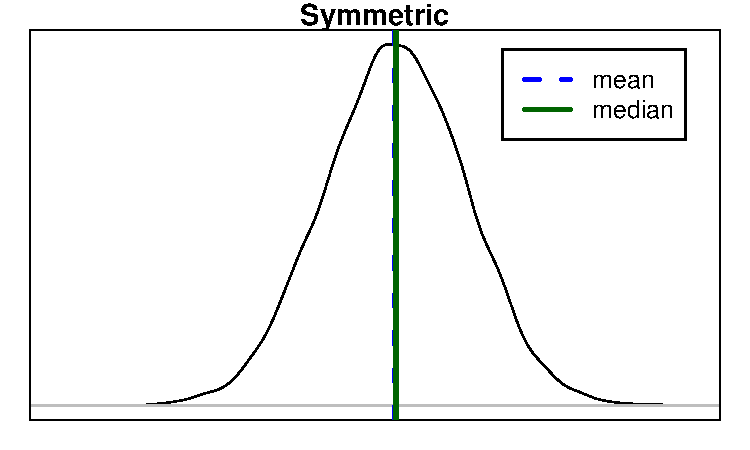
\includegraphics[width=0.33\textwidth]{2-1_numerical_data/figures/mean_med/sym}
\end{center}

\item 分布が歪んでいるか極端な外れ値がある場合、中心はしばしば中央値として定義される
\begin{itemize}
\item 右歪み：平均 $>$ 中央値
\item 左歪み：平均 $<$ 中央値 \\
\end{itemize}

\end{itemize}

\begin{center}
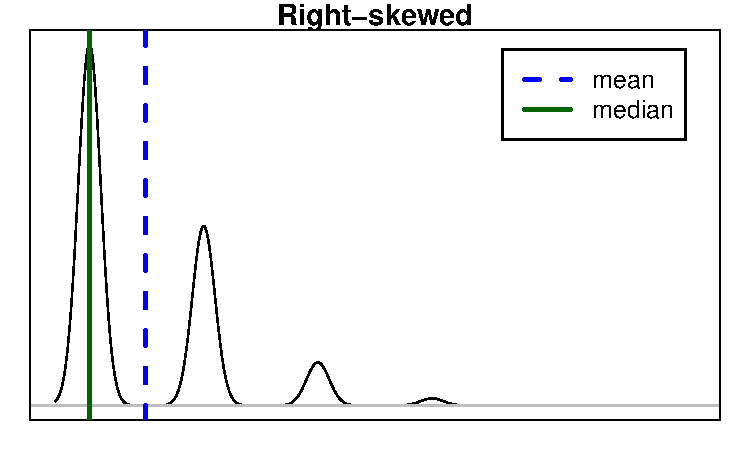
\includegraphics[width=0.33\textwidth]{2-1_numerical_data/figures/mean_med/rs}
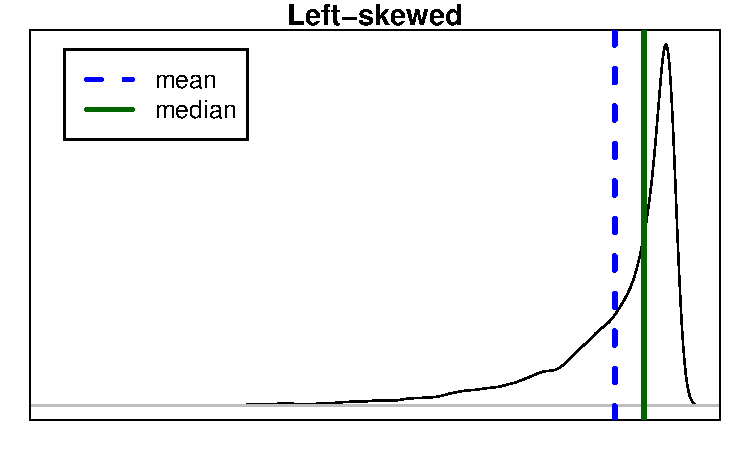
\includegraphics[width=0.33\textwidth]{2-1_numerical_data/figures/mean_med/ls}\\
\end{center}

\end{frame}

%%%%%%%%%%%%%%%%%%%%%%%%%%%%%%%%%%%%%

\begin{frame}
\frametitle{練習問題}

\pq{{\small 授業中にノートを取ることに費やした時間の割合（FacebookやTwitterなどと比較した）の分布について最も正しいと思われるのはどれか？}}

\vspace{-0.5cm}

\begin{columns}
\column{0.7\textwidth}
\begin{center}
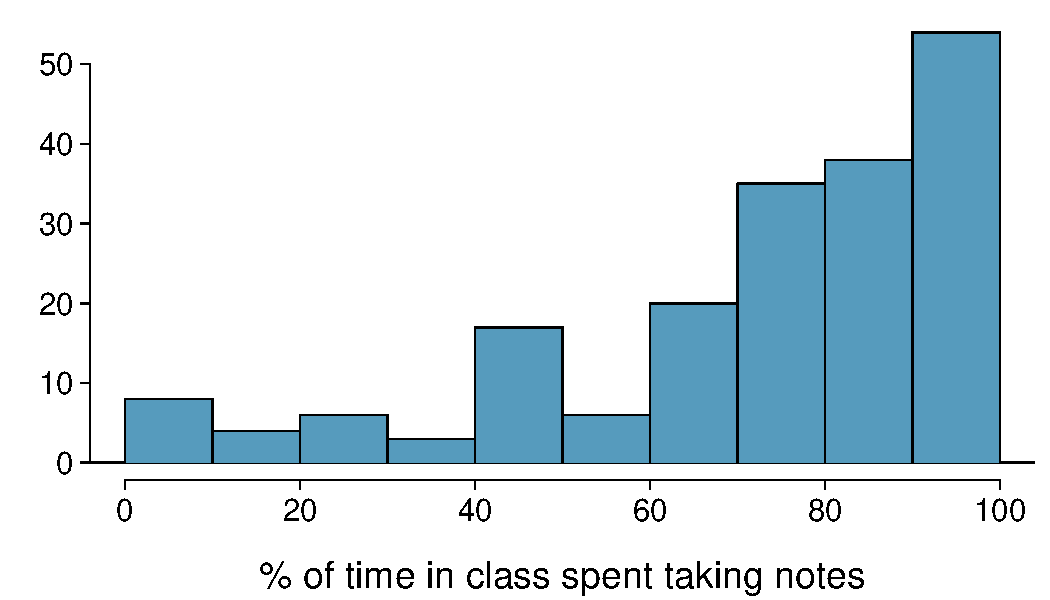
\includegraphics[width=0.9\textwidth]{2-1_numerical_data/figures/notes_perc/notes_perc_hist}
\end{center}
\column{0.3\textwidth}
$\:$ \\
$\:$ \\
\only<2->{\orange{中央値：80\% \\ 平均：76\%}}
\end{columns}

{\small
\begin{multicols}{2}
\begin{enumerate}[(a)]
\item 平均 $>$ 中央値
\solnMult{平均 $<$ 中央値}
\item 平均 $\approx$ 中央値
\item 判断不可能
\end{enumerate}
\end{multicols}
}

\end{frame}

%%%%%%%%%%%%%%%%%%%%%%%%%%%%%%%%%%%%%

\subsection{データの変換}

%%%%%%%%%%%%%%%%%%%%%%%%%%%%%%%%%%%%

\begin{frame}
\frametitle{極端に歪んだデータ}

データが極端に歪んでいる場合、変換すると分析しやすくなることがある。一般的な変換は\hl{対数変換}である。

左のヒストグラムは学生が観戦したバスケットボールの試合数の分布を示す。右のヒストグラムは試合数の対数の分布を示す。

\begin{center}
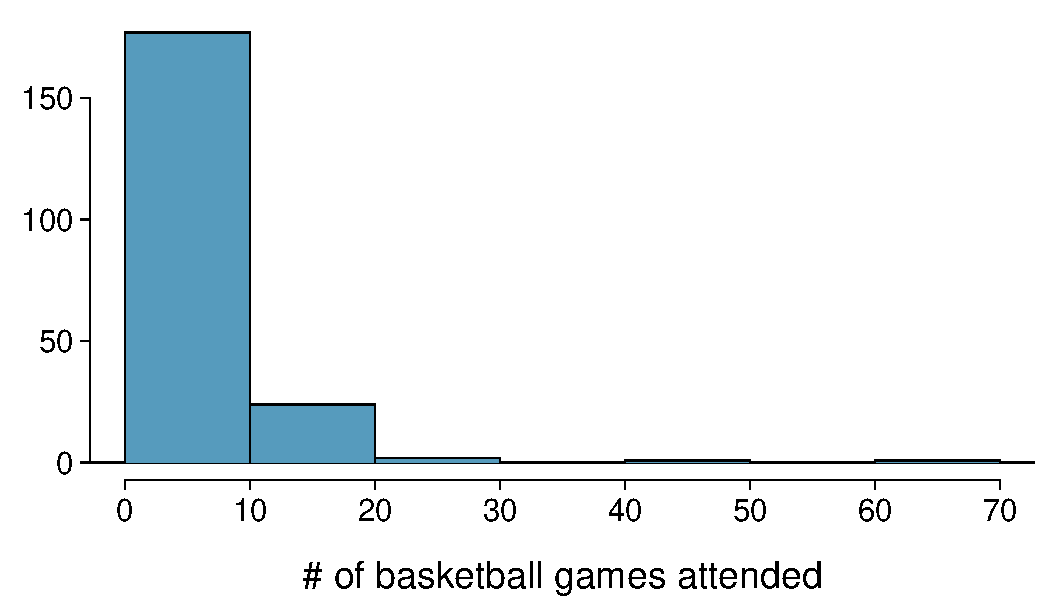
\includegraphics[width=0.45\textwidth]{2-1_numerical_data/figures/basket_games/basket_games_hist}
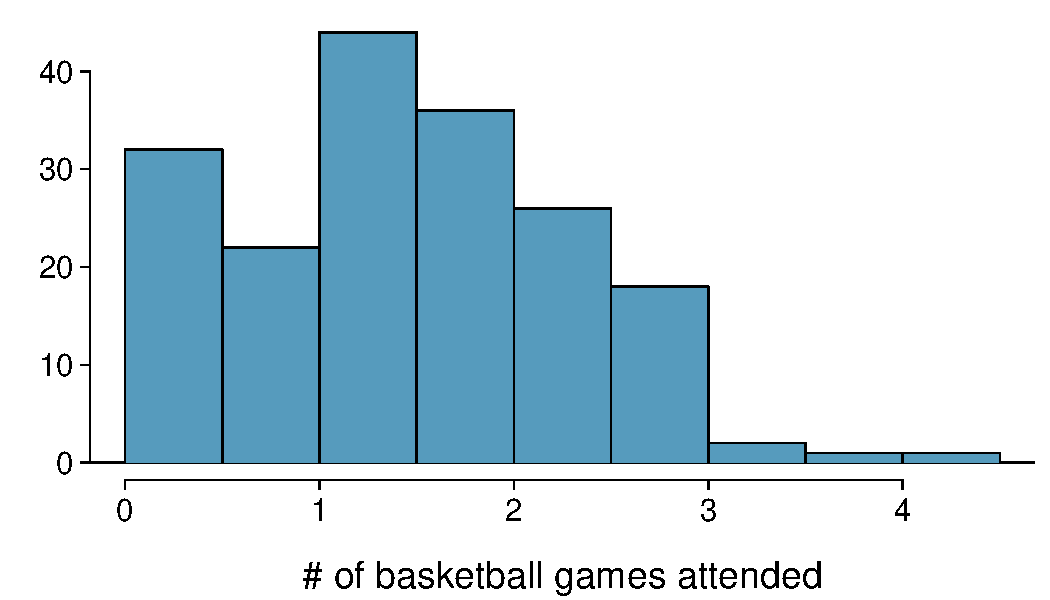
\includegraphics[width=0.45\textwidth]{2-1_numerical_data/figures/basket_games/basket_games_hist_log}
\end{center}

\end{frame}

%%%%%%%%%%%%%%%%%%%%%%%%%%%%%%%%%%%%

\begin{frame}
\frametitle{変換の利点と欠点}

\begin{itemize}

\item 歪んだデータは適切な変換によって外れ値が目立たなくなるため、変換後の方が分析しやすい。 \\
$\:$ \\
\renewcommand{\arraystretch}{1.5}
\begin{tabular}{l r r r r }
試合数		& 70 	& 50 		& 25 	& $\cdots$ \\
log（試合数）	& 4.25	& 3.91 	& 3.22	& $\cdots$
\end{tabular}

$\:$ \\

\item ただし、測定変数の対数単位での分析結果は解釈が難しいことがある。

\end{itemize}

\dq{他にどのような変数が極端に歪むと予想されるか？}

\soln{給与、住宅価格など。}

\end{frame}

%%%%%%%%%%%%%%%%%%%%%%%%%%%%%%%%%%%%

\subsection{データのマップ表示}

%%%%%%%%%%%%%%%%%%%%%%%%%%%%%%%%%%%%

\begin{frame}
\frametitle{強度マップ}

\dq{2000年から2010年にかけての人口変化において、どのようなパターンが見られるか？}

\begin{center}
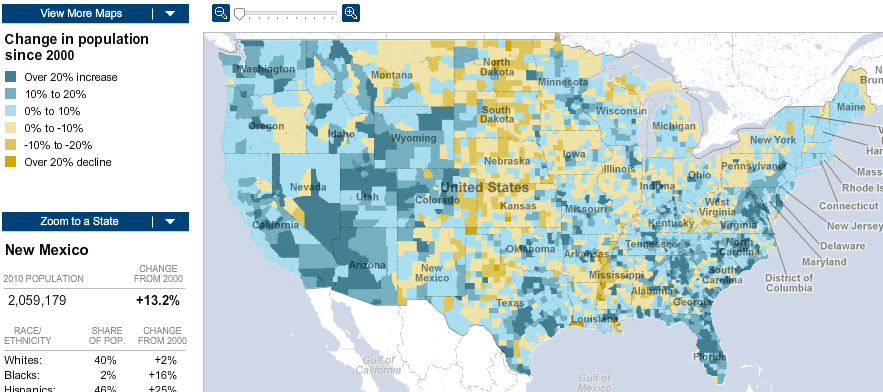
\includegraphics[width=0.95\textwidth]{2-1_numerical_data/figures/change_in_pop_intensity}
\end{center}

\ct{\webURL{http://projects.nytimes.com/census/2010/map}}

\end{frame}


%%%%%%%%%%%%%%%%%%%%%%%%%%%%%%%%%%%%
